\section{Introduction}
\label{sec:introduction}
  Keyphrases are single or multi-word expressions that represent the main topics
  of a document. Keyphrases are useful in many tasks such as information
  retrieval~\cite{medelyan2008smalltrainingset}, document
  summarization~\cite{litvak2008graphbased} or document
  clustering~\cite{han2007webdocumentclustering}. Although scientific articles
  usually provide them, most of the documents have no associated keyphrases.
  Therefore, the problem of automatically assigning keyphrases to documents is
  an active field of research.

  Automatic keyphrase extraction methods are divided into two categories:
  supervised and unsupervised methods. Supervised methods recast keyphrase
  extraction as a binary classification task~\cite{witten1999kea}, whereas
  unsupervised methods apply different kinds of techniques such as
  language modeling~\cite{tomokiyo2003languagemodel},
  clustering~\cite{liu2009keycluster} or graph-based
  ranking~\cite{mihalcea2004textrank}.

  In this paper, we present a new unsupervised method called TopicRank. This new
  method is an improvement of the TextRank method applied to keyphrase
  extraction~\cite{mihalcea2004textrank}. In the TextRank method, a document is
  represented by a graph where words are vertices and edges represent
  co-occurrence relations. A graph-based ranking model derived from
  PageRank~\cite{brin1998pagerank} is then used to assign a significance score
  to each word. Here, we propose to represent a document as a complete graph
  where vertices are not words but topics. We define a topic as a cluster of
  similar single and multi-word expressions.

  Our approach has several advantages over TextRank. Intuitively, ranking topics
  instead of words is a more straightforward way to identify the set of
  keyphrases that covers the main topics of a document. To do so, we simply
  select a keyphrase candidate from each of the top-ranked clusters. Clustering
  keyphrase candidates into topics also eliminates redundancy while reinforcing
  edges. This is very important because the ranking performance strongly depends
  on the conciseness of the graph, as well as its ability to precisely represent
  semantic relations within a document. Hence, another advantage of our approach
  is the use of a complete graph that better captures the semantic relations
  between topics.

  To evaluate TopicRank, we follow \newcite{hassan2010conundrums} who stated
  that multiple datasets must be used to evaluate and fully understand the
  strengths and weaknesses of a method. We use four evaluation datasets of
  different languages, document sizes and domains, and compare the keyphrases
  extracted by TopicRank against three baselines (TF-IDF and two graph-based
  methods). TopicRank outperforms the baselines on three of the datasets. As for
  the fourth one, an additional experiment shows that an improvement could be
  achieved with a more effective selection strategy.

  The rest of this paper is organized as follows. Section~\ref{sec:related_work}
  presents the existing methods for the keyphrase extraction task,
  Section~\ref{sec:clusterrank_approach} details our proposed approach,
  Section~\ref{sec:experimental_settings} describes the evaluation process and
  Section~\ref{sec:results} shows the analyzed results. Finally,
  Section~\ref{sec:conclusion_and_future_work} concludes this work and suggests
  directions for future work.

\section{Related Work}
\label{sec:related_work}
  The task of automatic keyphrase extraction has been well studied and many
  supervised and unsupervised approaches have been proposed. For supervised
  methods, keyphrase extraction is often treated as a binary classification
  task~\cite{witten1999kea}. Unsupervised approaches proposed so far have
  involved a number of techniques, including language
  modeling~\cite{tomokiyo2003languagemodel},
  clustering~\cite{liu2009keycluster} and graph-based
  ranking~\cite{mihalcea2004textrank}. While supervised approaches have
  generally proven to be more successful, the need for training data and the
  bias towards the domain on which they are trained remain two critical issues.

  In this paper, we concentrate on graph-based ranking methods for keyphrase
  extraction. Starting with TextRank~\cite{mihalcea2004textrank}, these methods
  are becoming the most widely used unsupervised approaches for keyphrase
  extraction. In TextRank, a document is represented as a graph in which
  vertices are words connected if they co-occur in a given window of words. The
  significance of each vertex is computed using a random walk algorithm derived
  from PageRank~\cite{brin1998pagerank}. Words corresponding to the top ranked
  vertices are then selected and assembled to generate keyphrases.

  \newcite{wan2008expandrank} propose SingleRank, a simple modification of
  TextRank that weights the edges with the number of co-occurrences and no
  longer extracts keyphrases by assembling ranked words. Keyphrases are noun
  phrases extracted from the document and ranked according to the sum of the
  significance of the words they contain. Although it improves the results, this
  scoring method has no proper justification and tends to assign high scores to
  long but non important phrases. For example, ``nash equilibrium'', from the
  file \textit{J-14.txt} of our evaluation dataset named SemEval, is a keyphrase
  composed of the two most significant words in the document, according to
  SingleRank. Therefore, SingleRank succeeds to extract it, but candidates such
  as ``unique nash equilibrium'' or ``exact nash equilibrium'' which are longer,
  then have a better score, are extracted too. With TopicRank, we aim to
  circumvent this by ranking clusters of single and multi-word expressions
  instead of words.

  \newcite{wan2008expandrank} use a small number of nearest neighbor documents
  to compute more accurate word co-occurrences and reinforce edge weights in the
  word graph. Borrowing co-occurrence information from multiple documents, their
  approach improves the word ranking performance. Instead of using words,
  \newcite{liang2009querylog} use keyphrase candidates as vertices. Applied to
  Chinese, their method uses query log knowledge to determine phrase boundaries.
  \newcite{tsatsaronis2010semanticrank} propose to connect vertices employing
  semantic relations computed using WordNet~\cite{miller1995wordnet} or
  Wikipedia. They also experiment with different random walk algorithms, such as
  HITS~\cite{kleinberg1999hits} or modified PageRank.

  \newcite{liu2010topicalpagerank} consider the topics of words using a Latent
  Dirichlet Allocation model~\cite[LDA]{blei2003lda}. As done by
  \newcite{haveliwala2003topicsensitivepagerank} for Information Retrieval, they
  propose to decompose PageRank into multiple PageRanks specific to various
  topics. A topic-biased PageRank is computed for each topic and corresponding
  word scores are combined. As this method uses a LDA model, it requires
  training data. With TopicRank, we also consider topics, but our aim is to use
  a single document, the document to be analyzed.

\section{TopicRank}
\label{sec:clusterrank_approach}
  TopicRank is an unsupervised method that aims to extract keyphrases from the
  most important topics of a document. Topics are defined as clusters of similar
  keyphrase candidates. Extracting keyphrases from a document consists in the
  following steps, illustrated in Figure~\ref{fig:processing_steps}. First, the
  document is preprocessed (sentence segmentation, word tokenization and
  Part-of-Speech tagging) and keyphrase candidates are clustered into topics.
  Then, topics are ranked according to their importance in the document and
  keyphrases are extracted by selecting one keyphrase candidate for each of the
  most important topics.
  \begin{figure}
    \centering
    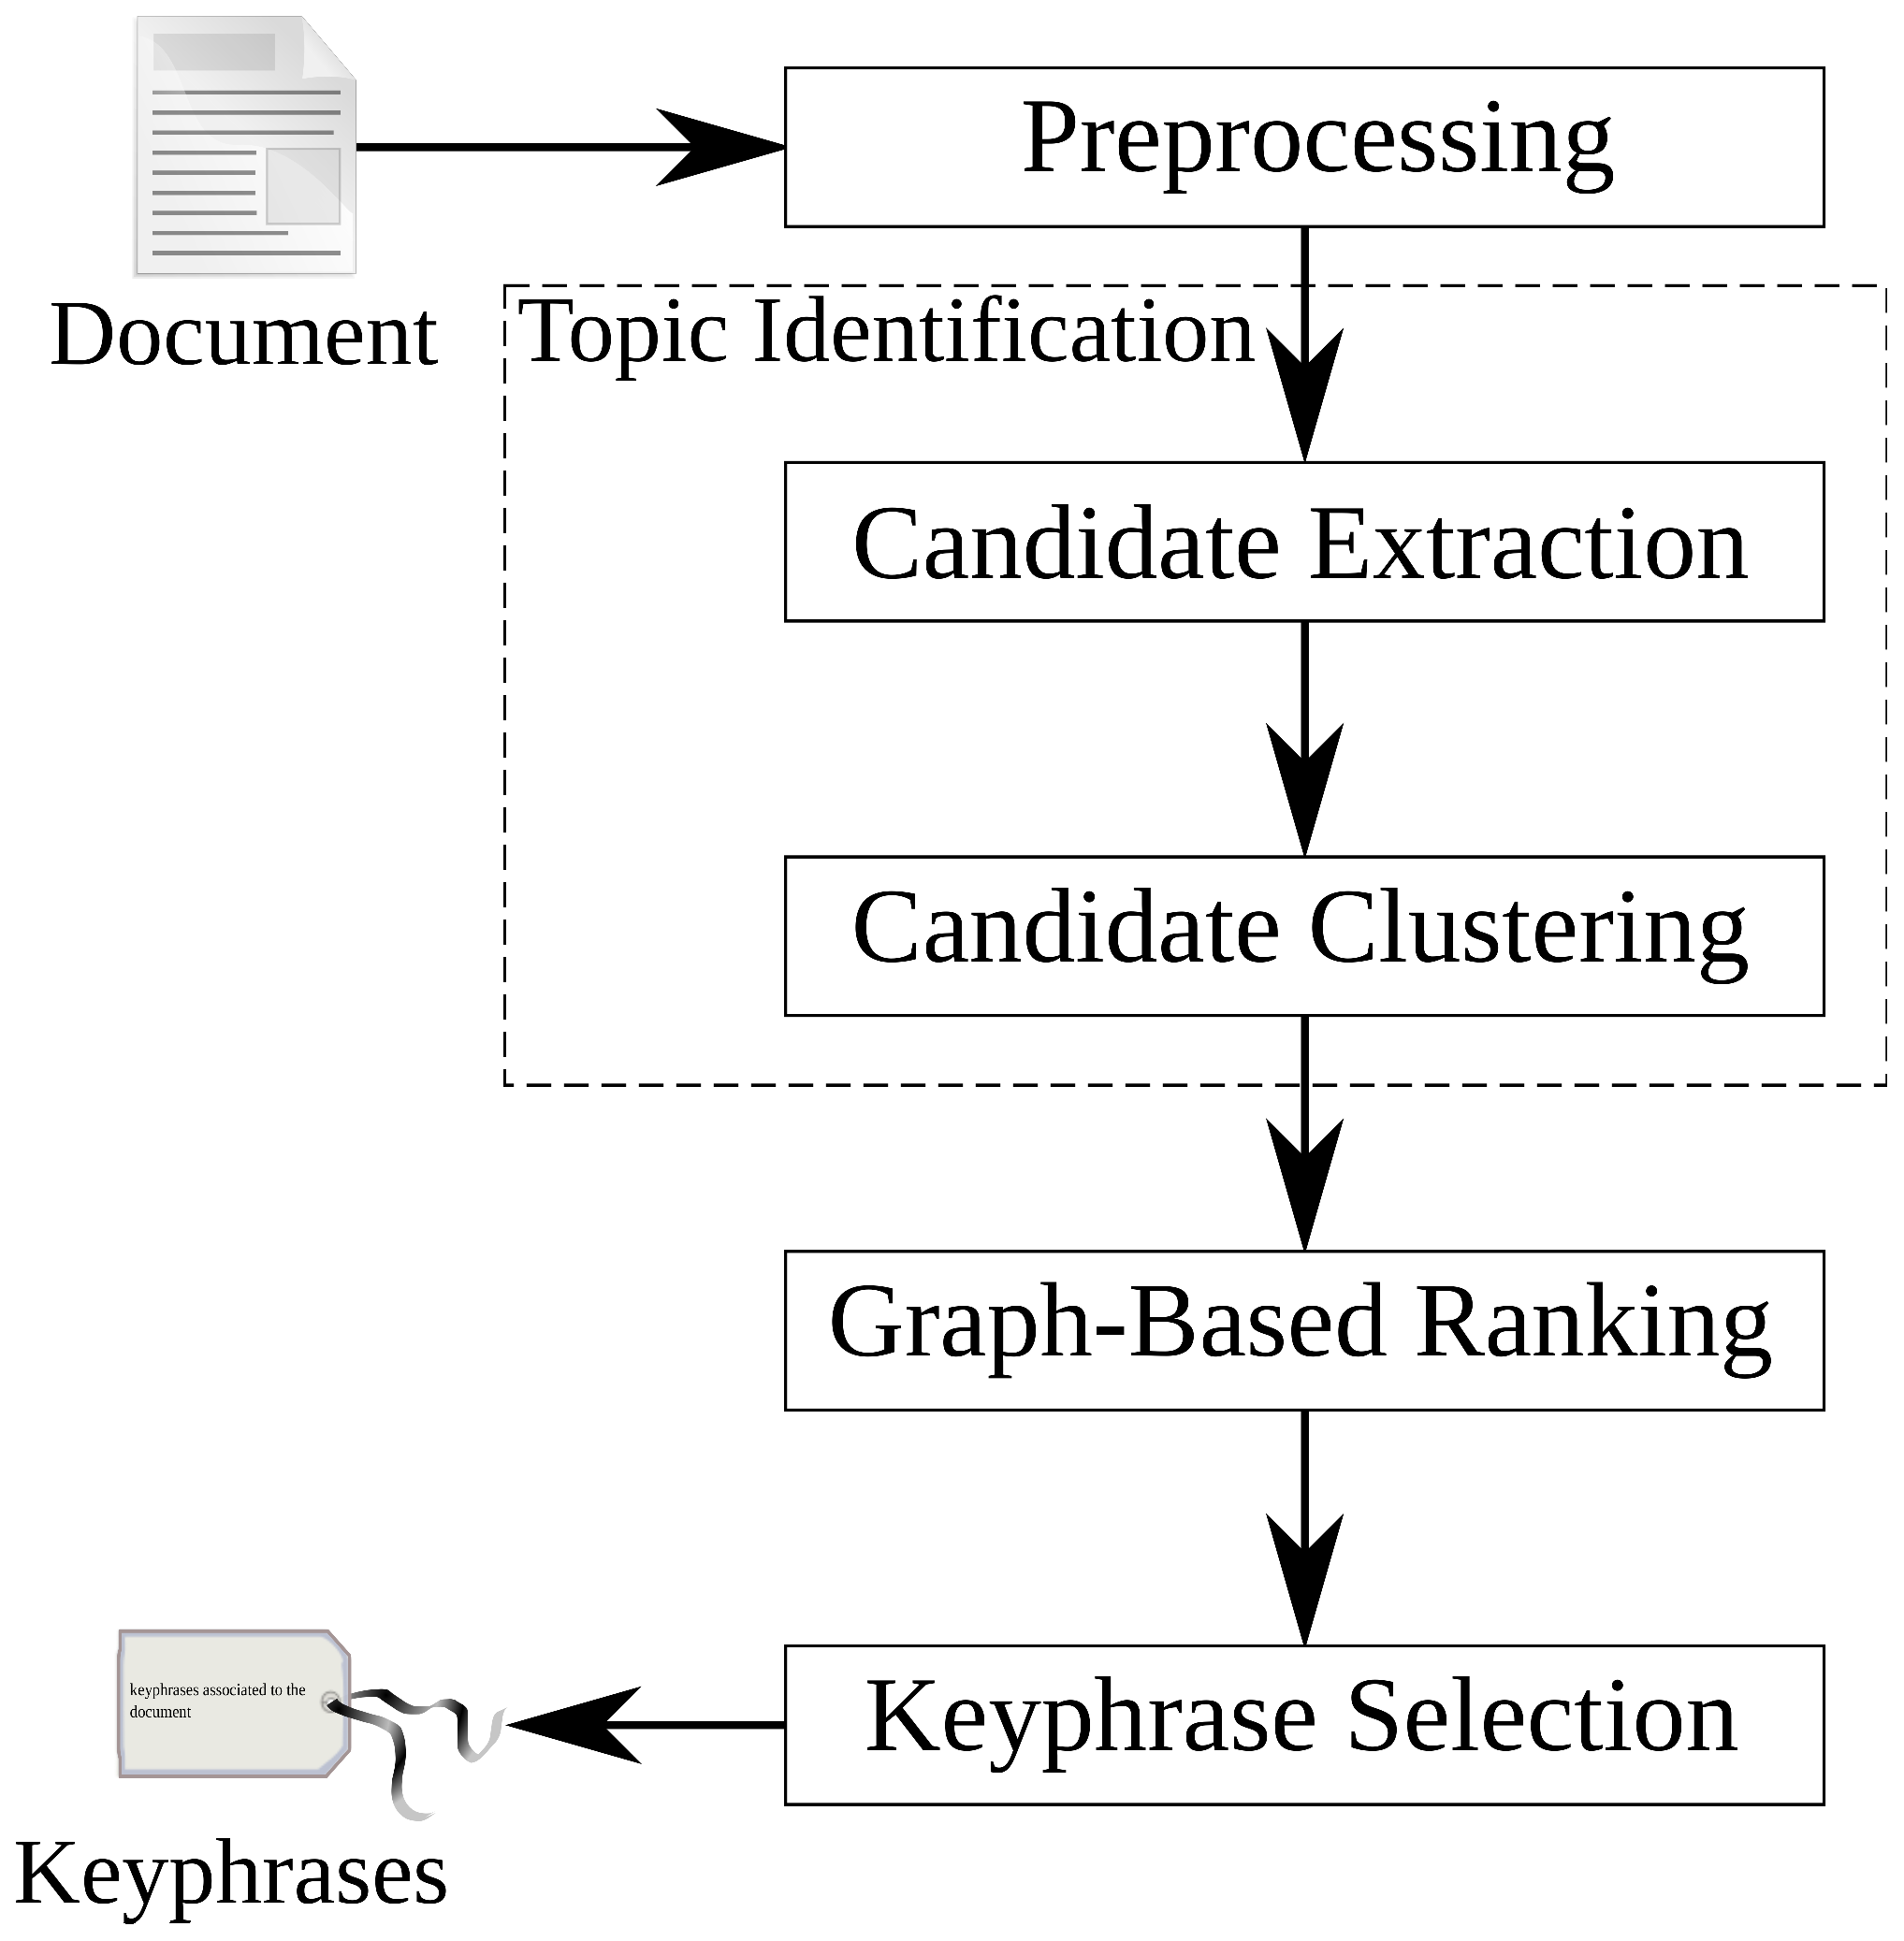
\includegraphics[width=0.35\textwidth]{include/processing_steps.eps}
    \caption{Processing steps of TopicRank. \label{fig:processing_steps}}
  \end{figure}

  Section~\ref{subsec:subjects_identification} first explains how the topics are
  identified within a document, section~\ref{subsec:graph_based_ranking}
  presents the approach we use to rank them and
  section~\ref{subsec:keyphrase_selection} describes the keyphrase selection.

  \subsection{Topic Identification}
  \label{subsec:subjects_identification}
    Keyphrases describe the most important topics of a document, thus the first
    step is to identify the keyphrase candidates that represent them.
    \newcite{hulth2003keywordextraction} stated that most keyphrases assigned
    by human readers are noun phrases. Hence, the most important topics of a
    document can be found by extracting their most significant noun phrases.
    We follow \newcite{wan2008expandrank} and extract the longest sequences of
    nouns and adjectives from the document as keyphrase candidates. Other
    methods use syntactically filtered n-grams that are most likely to contain a
    larger number of candidates matching with reference keyphrases, but the
    n-gram restricted length is a problem. Indeed, n-grams do not always capture
    as much information as the longest noun phrases. Also, they are less likely
    to be grammatically correct.

    In a document, a topic is usually conveyed by more than one noun phrase.
    Consequently, some keyphrase candidates are redundant in regard to the topic
    they represent. Existing graph-based methods (TextRank, SingleRank, etc.) do
    not take that fact into account. Keyphrase candidates are usually treated
    independently and the information about the topic they represent is
    scattered throughout the graph. Thus, we propose to group similar noun
    phrases as a single entity, a topic.

    We consider that two keyphrase candidates are similar if they have at least
    25\% of overlapping words\footnote{The value of 25\% has been defined
    empirically.}. Keyphrase candidates are stemmed to reduce their inflected
    word forms into root forms\footnote{We chose to use stems because of the
    availability of stemmers for various languages, but using lemmas is another
    possibility that could probably work better.}. To automatically group
    similar candidates into topics, we use a Hierarchical Agglomerative
    Clustering (HAC) algorithm. Among the commonly used linkage strategies,
    which are complete, average and single linkage, we use the average linkage,
    because it stands as a compromise between complete and single linkage. In
    fact, using a highly agglomerative strategy such as complete linkage is more
    likely to group topically unrelated keyphrase candidates, whereas a strategy
    such as single linkage is less likely to group topically related keyphrase
    candidates.

  \subsection{Graph-Based Ranking}
  \label{subsec:graph_based_ranking}
    TopicRank represents a document by a complete graph in which topics are
    vertices and edges are weighted according to the strength of the semantic
    relations between vertices. Then, TextRank's graph-based ranking model is
    used to assign a significance score to each topic.

    \begin{figure*}
      \centering
      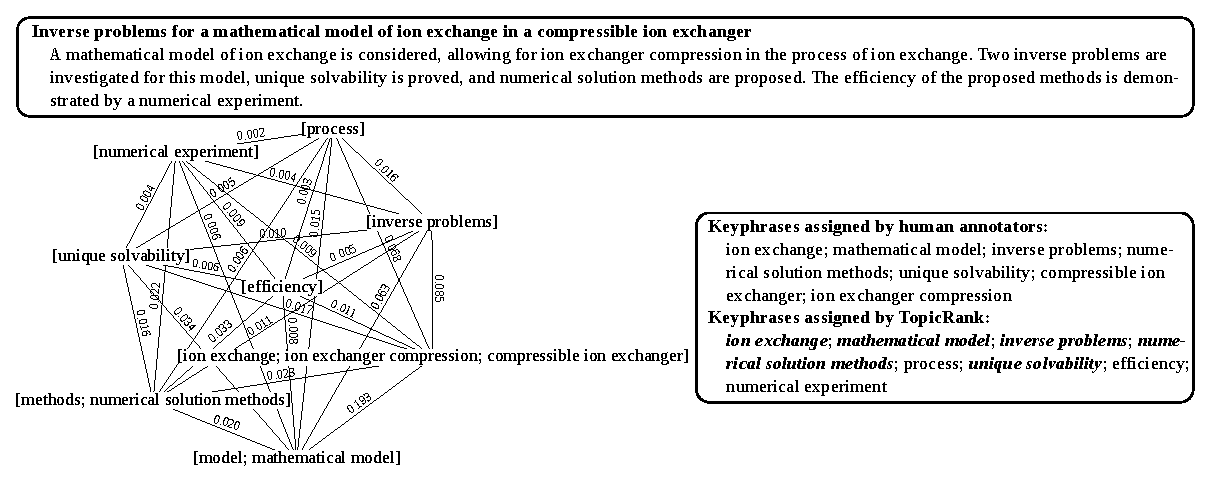
\includegraphics[width=\textwidth]{include/2040_full.eps}
      \caption{Sample graph build by TopicRank from Inspec, file
               \textit{2040.abstr}. \label{fig:topicrank}}
    \end{figure*}

    \subsubsection{Graph Construction}
    \label{subsubsec:graph_construction}
      Formally, let $G = (V, E)$ be a complete and undirected graph where $V$ is
      a set of vertices and the edges $E$ a
      subset\footnote{$E = \{(v_1, v_2)\ |\ \forall v_1, v_2 \in V,\ v_1 \neq v_2\}$}
      of $V \times V$. Vertices are topics and the edge between two topics $t_i$
      and $t_j$ is weighted according to the strength of their semantic
      relation. $t_i$ and $t_j$ have a strong semantic relation if their
      keyphrase candidates often appear close to each other in the document.
      Therefore, the weight $w_{i, j}$ of their edge is defined as follows:
      \begin{align}
        w_{i, j} &= \mathlarger{\sum}_{c_i \in t_i}\ \mathlarger{\sum}_{c_j \in t_j} \text{dist}(c_i, c_j) \label{math:semantic_relatedness}\\
        \text{dist}(c_i, c_j) &= \sum_{p_i \in \text{pos}(c_i)}\ \sum_{p_j \in \text{pos}(c_j)} \frac{1}{|p_i - p_j|} \label{math:distance}
      \end{align}
      where $\text{dist}(c_i, c_j)$ refers to the reciprocal distances between
      the offset positions of the candidate keyphrases $c_i$ and $c_j$ in the
      document and where $\text{pos}(c_i)$ represents all the offset positions
      of the candidate keyphrase $c_i$.

      Our approach to construct the graph differs from TextRank. $G$ is a
      complete graph and topics are therefore interconnected. The completeness
      of the graph has the benefit of providing a more exhaustive view of the
      relations between topics. Also, computing weights based on the distances
      between offset positions bypasses the need for a manually defined
      parameter, such as the window of words used by state-of-the-art methods
      (TextRank, SingleRank, etc).

      Figure~\ref{fig:topicrank} shows a sample graph built for an abstract from
      one of our evaluation datasets (Inspec). Vertices are topics, represented
      as clusters of lexically similar keyphrase candidates, and connected with
      all the others. In the example, we see the naivety of our clustering
      approach. Indeed, the clustering succeeds to group ``ion exchanger'',
      ``ion exchanger compression'' and ``compressible ion exchanger'', but the
      clustering of ``methods'' with ``numerical solution methods'' and
      ``model'' with ``mathematical model'' may be ambiguous as ``methods'' and
      ``model'' can be used to refer to other methods or models.

    \subsubsection{Subject Ranking}
    \label{subsubsec:ranking}
      Once the graph is created, the graph-based ranking model TextRank,
      proposed by \newcite{mihalcea2004textrank}, is used to rank the topics.
      This model assigns a significance score to topics based on the concept of
      ``voting'': high-scoring topics contribute more to the score of their
      connected topic $t_i$:
      \begin{align}
        S(t_i) = (1 - \lambda) + \lambda \times \sum_{t_j \in V_i} \frac{w_{j, i} \times S(t_j)}{\mathlarger{\sum}_{t_k \in V_j} w_{j, k}} \label{math:textrank}
      \end{align}
      where $V_i$ are the topics voting for $t_i$ and $\lambda$ is a damping
      factor generally defined to 0.85~\cite{brin1998pagerank}.

  \subsection{Keyphrase Selection}
  \label{subsec:keyphrase_selection}
    Keyphrase selection is the last step of TopicRank. For each topic, only the
    most representative keyphrase candidate is selected. This selection avoids
    redundancy and leads to a good coverage of the document topics, because
    extracting $k$ keyphrases precisely covers $k$ topics.

    To find the candidate that best represents a topic, we propose three
    strategies. Assuming that a topic is first introduced by its generic form,
    the first strategy is to select the keyphrase candidate that appears first
    in the document. The second strategy assumes that the generic form of a
    topic is the one that is most frequently used and the third strategy selects
    the centroid of the cluster. The centroid is the candidate that is the most
    similar to the other candidates of the cluster\footnote{The similarity
    between two candidates is computed with the stem overlap measure used by the
    clustering algorithm.}.

\section{Experimental Settings}
\label{sec:experimental_settings}
  \subsection{Datasets}
  \label{subsec:datasets}
    \begin{table*}
      \centering
      \begin{tabular}{@{ }rccccccc@{ }}
        \toprule
        \multirow{2}{*}[-2pt]{\textbf{Corpus}} & \multicolumn{4}{c}{\textbf{Documents}} & \multicolumn{3}{c}{\textbf{Keyphrases}}\\
        \cmidrule(lr){2-5}\cmidrule(l){6-8}
        & Type & Language & Number & Tokens average & Total & Average & Missing\\
        \midrule
        Inspec & Abstracts & English & 500 & $~~$136.3 & 4913 & $~~$9.8 & 21.8\%\\
        SemEval & Papers & English & 100 & 5179.6 & 1466 & 14.7 & 19.3\%\\
        WikiNews & News & French & 100 & $~~$309.6 & $~~$964 & $~~$9.6 & $~~$4.4\%\\
        DEFT & Papers & French & $~~$93 & 6844.0 & $~~$485 & $~~$5.2 & 18.2\%\\
        \bottomrule
      \end{tabular}
      \caption{Dataset statistics (missing keyphrases are counted based on
               their stemmed form). \label{tab:corpora}}
    \end{table*}

    To compare the keyphrases extracted by TopicRank against existing methods,
    we employ four standard evaluation dataset of different languages, document
    sizes and domains.
    
    The first dataset, formerly used by \newcite{hulth2003keywordextraction},
    contains 2000 English abstracts of journal papers from the Inspec database.
    The 2000 abstracts are divided into three sets: a training set, which
    contains 1000 abstracts, a validation set containing 500 abstracts and a
    test set containing the 500 remaining abstracts. In our experiments we use
    the 500 abstracts from the test set. Several reference keyphrase sets are
    available with this dataset. Just as \newcite{hulth2003keywordextraction},
    we use the uncontrolled reference, created by professional indexers.

    The second dataset was built by \newcite{kim2010semeval} for the keyphrase
    extraction task of the SemEval 2010 evaluation campaign. This dataset is
    composed of 284 scientific articles (in English) from the ACM Digital
    Libraries (conference and workshop papers). The 284 documents are
    divided into three sets: a trial set containing 40 documents, a training
    set, which contains 144 documents and a test set containing 100 documents.
    In our experiments we use the 100 documents of the test set. As for the
    reference keyphrases, we use the combination of author and reader assigned
    keyphrases provided by \newcite{kim2010semeval}.

    The third dataset is a French corpus that we created from the French version
    of WikiNews\footnote{The WikiNews dataset is available for free at the given
    url: \url{https://github.com/adrien-bougouin/WikinewsKeyphraseCorpus}.}. It
    contains 100 news articles published between May 2012 and December 2012.
    Each document has been annotated by at least three students. We combined the
    annotations of each document and removed the lexical redundancies. All of
    the 100 documents are used in our experiments.

    The fourth dataset is a French corpus made for the keyphrase extraction task
    of the DEFT 2012 evaluation campaign~\cite{paroubek2012deft}. It contains
    468 scientific articles extracted from Érudit. These documents are used for
    two tasks of DEFT and are, therefore, divided in two datasets of 244
    documents each. In our experiments we use the test set of the second task
    dataset. It contains 93 documents provided with author keyphrases.

    Table~\ref{tab:corpora} gives statistics about the datasets. They are
    different in terms of document sizes and number of assigned keyphrases. The
    Inspec and WikiNews datasets have shorter documents (abstract and news
    articles) compared to SemEval and DEFT that both contain full-text
    scientific articles. Also, the keyphrases provided with the datasets are not
    always present in the documents (less than 5\% of missing keyphrases for
    Wikinews and about 20\% of missing keyphrases for the other datasets). This
    induces a bias in the results. As explained by
    \newcite{hassan2010conundrums}, some researchers avoid this problem by
    removing missing keyphrases from the references. In our experiments, missing
    keyphrases have not been removed. However, we evaluate with stemmed forms of
    candidates and reference keyphrases to reduce mismatches.

  \subsection{Preprocessing}
  \label{subsec:pre_processing}
    For each dataset, we apply the following preprocessing steps: sentence
    segmentation, word tokenization and Part-of-Speech tagging. For word
    tokenization, we use the TreebankWordTokenizer provided by the python
    Natural Language ToolKit~\cite{bird2009nltk} for English and the Bonsai word
    tokenizer\footnote{The Bonsai word tokenizer is a tool provided with the
    Bonsai PCFG-LA parser:
    \url{http://alpage.inria.fr/statgram/frdep/fr_stat_dep_parsing.html}.} for
    French. For Part-of-Speech tagging, we use the Stanford
    POS-tagger~\cite{toutanova2003stanfordpostagger} for English and
    MElt~\cite{denis2009melt} for French.

  \subsection{Baselines}
  \label{subsec:baselines}
    \begin{table*}
      \centering
      \begin{tabular}{@{ }rcccccccccccc@{ }}
        \toprule
        \multirow{2}{*}[-2pt]{\textbf{Methods}} & \multicolumn{3}{c}{\textbf{Inspec}} & \multicolumn{3}{c}{\textbf{SemEval}} & \multicolumn{3}{c}{\textbf{WikiNews}} & \multicolumn{3}{c}{\textbf{DEFT}}\\
        \cmidrule(lr){2-4}\cmidrule(lr){5-7}\cmidrule(lr){8-10}\cmidrule(l){11-13}
        & P & R & F & P & R & F & P & R & F & P & R & F\\
        \midrule
        TF-IDF & 32.7 & 38.6 & 33.4$^{~}$ & 13.2 & $~~$8.9 & 10.5$^{~}$ & 33.9 & 35.9 & 34.3$^{~}$ & 10.3 & 19.1 & 13.2$^{~}$\\
        TextRank & 14.2 & 12.5 & 12.7$^{~}$ & $~~$7.9 & $~~$4.5 & $~~$5.6$^{~}$ & $~~$9.3 & $~~$8.3 & $~~$8.6$^{~}$ & $~~$4.9 & $~~$7.1 & $~~$5.7$^{~}$\\
        SingleRank & 34.8 & 40.4 & \textbf{35.2}$^{~}$ & $~~$4.6 & $~~$3.2 & $~~$3.7$^{~}$ & 19.4 & 20.7 & 19.7$^{~}$ & $~~$4.5 & $~~$9.0 & $~~$5.9$^{~}$\\
        TopicRank & 27.6 & 31.5 & 27.9  & 14.9 & 10.3 & \textbf{12.1}$^\dagger$ & 35.0 & 37.5 & \textbf{35.6}$^\dagger$ & 11.7 & 21.7 & \textbf{15.1}$^\dagger$\\
        \bottomrule
      \end{tabular}
      \caption{Comparison of TF-IDF, TextRank, SingleRank and TopicRank methods,
               when extracting a maximum of 10 keyphrases. Results are expressed
               as a percentage of precision (\text{P}), recall (\text{R}) and
               f-score (\text{F}). $\dagger$ indicates TopicRank's significant
               improvement over TextRank and SingleRank at 0.001 level using
               Student's t-test. \label{tab:results}}
    \end{table*}

    For comparison purpose, we use three baselines. The first baseline is
    TF-IDF~\cite{jones1972tfidf}, commonly used because of the difficulty to achieve competitive
    results against it~\cite{hassan2010conundrums}. This method relies on a
    collection of documents and assumes that the $k$ keyphrase candidates
    containing words with the highest TF-IDF weights are the keyphrases of the
    document. As TopicRank aims to be an improvement of the state-of-the-art
    graph-based methods for keyphrase extraction, the last two baselines are
    TextRank~\cite{mihalcea2004textrank} and
    SingleRank~\cite{wan2008expandrank}. In these methods, the graph is
    undirected, vertices are syntactically filtered words (only nouns and
    adjectives) and the edges are created based on the co-occurrences of words
    within a window of 2 for TextRank and 10 for SingleRank. As well as their
    window size, they differ in the weighting of the graph: TextRank has an
    unweighted graph and SingleRank has a graph weighted with the number of
    co-occurrences between the words. A graph-based ranking model derived from
    PageRank~\cite{brin1998pagerank} ranks each vertex and extracts multi-word
    keyphrases according to the ranked words. In TextRank, the $k$-best words
    are used as keyphrases and the adjacent sequences in the document are
    collapsed into multi-word keyphrases. Although $k$ is normally proportional
    to the number of vertices in the graph, we set it to a constant number,
    because experiments conducted by \newcite{hassan2010conundrums} show that
    the optimal value of the ratio depends on the size of the document. In
    SingleRank, noun phrases extracted with the same method as TopicRank are
    ranked by a score equal to the sum of their words scores. Then, the
    $k$-best noun phrases are selected as keyphrases.
    
    For all the baselines, we consider keyphrase candidates which have the same
    stemmed form as redundant. Once they are ranked we keep the best candidate
    and remove the others. This can only affect the results in a positive way,
    because the evaluation is performed with stemmed forms, which means that
    removed candidates are considered equal to the retained candidate.

  \subsection{Evaluation Measures}
  \label{subsec:measures}
    \begin{table*}
      \centering
      \begin{tabular}{@{ }rcccccccccccc@{ }}
        \toprule
        \multirow{2}{*}[-2pt]{\textbf{Methods}} & \multicolumn{3}{c}{\textbf{Inspec}} & \multicolumn{3}{c}{\textbf{SemEval}} & \multicolumn{3}{c}{\textbf{WikiNews}} & \multicolumn{3}{c}{\textbf{DEFT}}\\
        \cmidrule(lr){2-4}\cmidrule(lr){5-7}\cmidrule(lr){8-10}\cmidrule(l){11-13}
        & P & R & F & P & R & F & P & R & F & P & R & F\\
        \midrule
        SingleRank & 34.8 & 40.4 & 35.2 & $~~$4.6 & $~~$3.2 & $~~$3.7$^{~}$ & 19.4 & 20.7 & 19.7$^{~}$ & $~~$4.5 & $~~$9.0 & $~~$5.9$^{~}$\\
        +phrases & 21.5 & 25.9 & 22.1 & $~~$9.6 & $~~$7.0 & $~~$8.0$^\dagger$ & 28.6 & 30.1 & 28.9$^\dagger$ & 10.5 & 19.7 & 13.5$^\dagger$\\
        +topics & 26.6 & 30.2 & 26.8 & 14.7 & 10.2 & 11.9$^\dagger$ & 31.0 & 32.8 & 31.4$^\dagger$ & 11.5 & 21.4 & 14.8$^\dagger$\\
        +complete & 34.9 & 41.0 & \textbf{35.5} & $~~$5.5 & $~~$3.8 & $~~$4.4$^{~}$ & 20.0 & 21.4 & 20.3${~}$ & $~~$4.4 & $~~$9.0 & $~~$5.8$^{~}$\\
        TopicRank & 27.6 & 31.5 & 27.9  & 14.9 & 10.3 & \textbf{12.1}$^\dagger$ & 35.0 & 37.5 & \textbf{35.6}$^\dagger$ & 11.7 & 21.7 & \textbf{15.1}$^\dagger$\\
        \bottomrule
      \end{tabular}
      \caption{Comparison of the individual modifications from SingleRank to
               TopicRank, when extracting a maximum of 10 keyphrases. Results
               are expressed as a percentage of precision (\text{P}), recall
               (\text{R}) and f-score (\text{F}). $\dagger$ indicates a
               significant improvement over SingleRank at 0.001 level using
               Student's t-test.
               \label{tab:singlerank_improvements}}
    \end{table*}

    The performances of TopicRank and the baselines are evaluated in terms of
    precision, recall and f-score (f1-measure) when a maximum of 10 keyphrases
    are extracted ($k = 10$). As said before, the candidate and reference
    keyphrases are stemmed to reduce the number of mismatches.

\section{Results}
\label{sec:results}
  To validate our approach, we designed three experiments. The first experiment
  compares TopicRank\footnote{Results reported for TopicRank are obtained with
  the first position selection strategy.} to the baselines\footnote{TopicRank
  and the baselines implementations can be found at the given url:
  \url{https://github.com/adrien-bougouin/TopicRank/tree/ijcnlp_2013}.}, the
  second experiment individually evaluates the modifications of TopicRank
  compared to SingleRank\footnote{The second experiment is performed with
  SingleRank instead of TextRank, because SingleRank also uses a graph with
  weighted edges and is, therefore, closer to TopicRank.} and the last
  experiment compares the keyphrase selection strategies. To show that the
  clusters are well ranked, we also present the results that could be achieved
  with a ``perfect'' keyphrase selection strategy.

  Table~\ref{tab:results} shows the results of TopicRank and the three
  baselines. Overall, our method outperforms TextRank, SingleRank and TF-IDF.
  The results of TopicRank and the baselines are lower on SemEval and DEFT (less
  than 16\% of f-score), so we deduce that it is more difficult to treat long
  documents than short ones. On Inspec, TopicRank fails to do better than all
  the baselines, but on SemEval, WikiNews and DEFT, it performs better than
  TF-IDF and significantly outperforms TextRank and SingleRank. Also, we observe
  a gap between TF-IDF's and the two graph-based baselines results. Although
  TopicRank is a graph-based method, it overcomes this gap by almost tripling
  the f-score of both TextRank and SingleRank.

  Table~\ref{tab:singlerank_improvements} shows the individual modifications of
  TopicRank compared to SingleRank. We evaluate SingleRank when vertices are
  keyphrase candidates (+phrases), vertices are topics (+topics) and when
  TopicRank's graph construction is used with word vertices (+complete). Using
  keyphrase candidates as vertices significantly improves SingleRank on SemEval,
  WikiNews and DEFT. On Inspec, it induces a considerable loss of performance
  caused by an important deficit of connections that leads to connected
  components, as shown in Figure~\ref{fig:phrases_graph}. When we look at the
  distribution of ``fuzzy'' into the graph, we can see that it is scattered
  among the connected components and, therefore, increases the difficulty to
  select ``fuzzy Bayesian inference techniques'' as a keyphrase (according to
  the reference). The other datasets contain longer documents, which may dampen
  this problem. Overall, using topics as vertices performs better than using
  keyphrase candidates. Using topics significantly outperforms SingleRank on
  SemEval, WikiNews and DEFT. As for the new graph construction, SingleRank is
  improved on Inspec, SemEval and WikiNews. Results on DEFT are lower than
  SingleRank, but still competitive. Although the improvements are not
  significant, the competitive results point out that the new graph construction
  can be used instead of the former method, which requires to manually define a
  window of words. Experiments show that the three contributions are
  improvements and TopicRank benefits from each of them.

  Table~\ref{tab:cluster_ranking_evaluation} shows the results of TopicRank when
  selecting either the first appearing candidate, the most frequent one or the
  centroid of each cluster. Selecting the first appearing keyphrase candidate is
  the best strategy of the three. It significantly outperforms the frequency and
  the centroid strategies on SemEval, WikiNews and DEFT. On SemEval and DEFT, we
  observe a huge gap between the results of the first position strategy and the
  others. The two datasets are composed of scientific articles where the full
  form of the main topics are often introduced at the beginning and then,
  conveyed by abbreviations or inherent concepts (e.g. the file
  \textit{C-17.txt} from SemEval contains \textit{packet-switched network} as a
  keyphrase where \textit{packet} is more utilized in the content). These are
  usually more similar to the generic form and/or more frequent, which explains
  the observed gap.

  \begin{figure}[h]
    \centering
    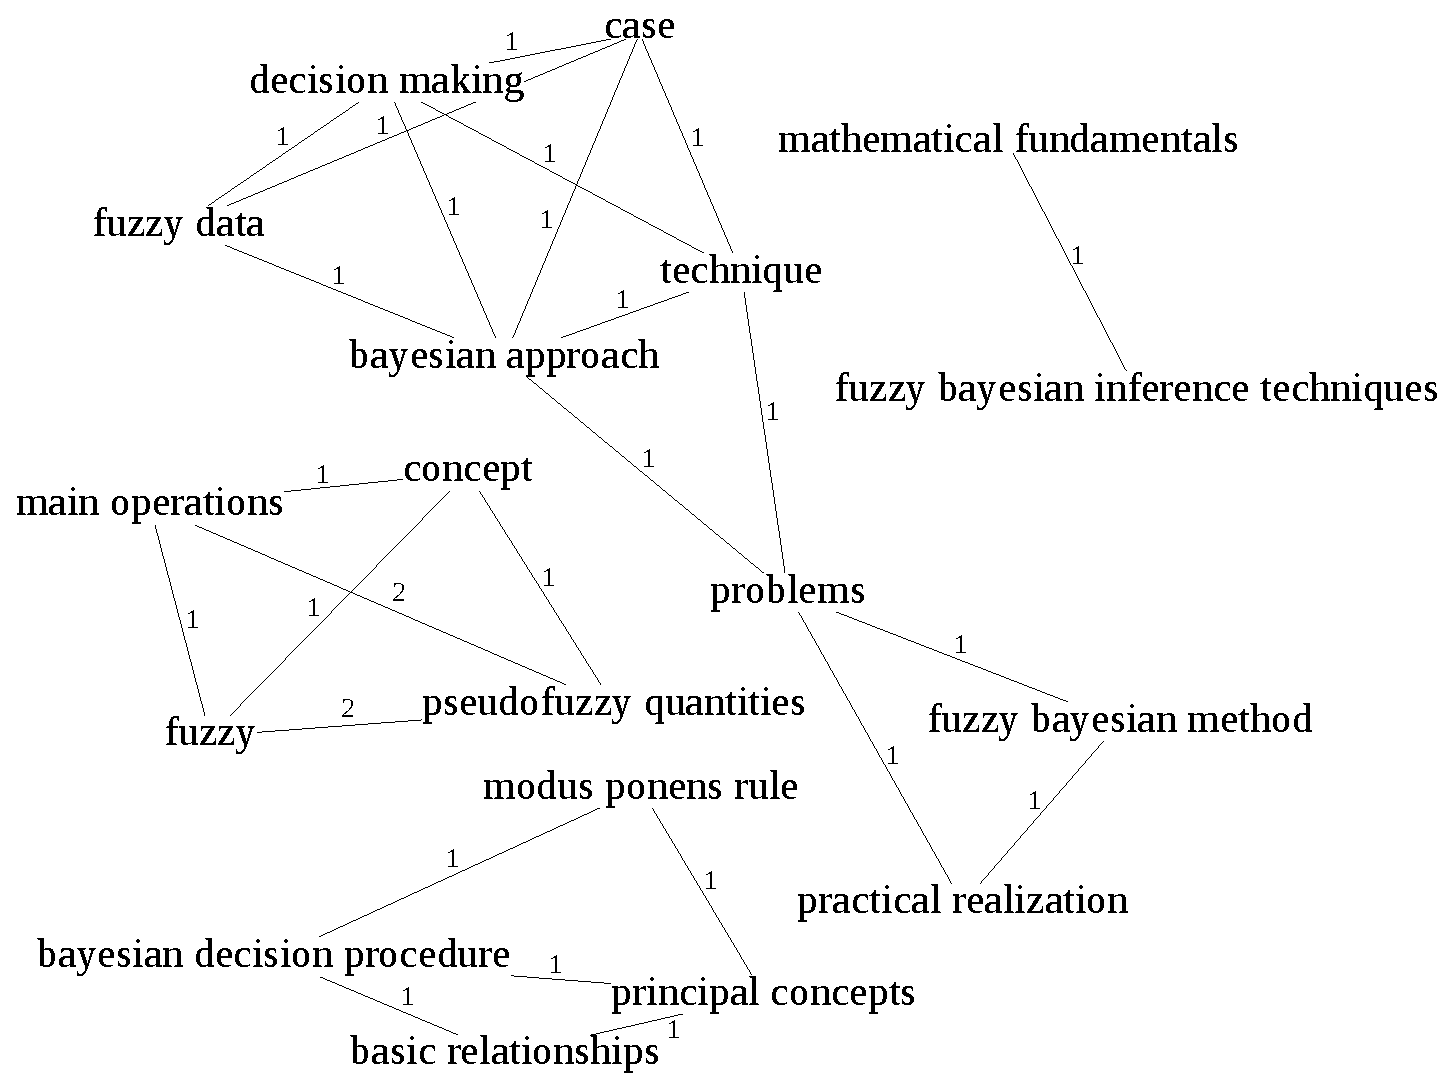
\includegraphics[width=.475\textwidth]{include/1931.eps}
    \caption{Connected component problem with the method SingleRank+phrases.
             Example taken from Inspec, file \textit{1931.abstr}.
             \label{fig:phrases_graph}}
  \end{figure}

  \begin{table*}
    \centering
    \begin{tabular}{@{ }rcccccccccccc@{ }}
      \toprule
      \multirow{2}{*}[-2pt]{\textbf{Methods}} & \multicolumn{3}{c}{\textbf{Inspec}} & \multicolumn{3}{c}{\textbf{SemEval}} & \multicolumn{3}{c}{\textbf{WikiNews}} & \multicolumn{3}{c}{\textbf{DEFT}}\\
      \cmidrule(lr){2-4}\cmidrule(lr){5-7}\cmidrule(lr){8-10}\cmidrule(l){11-13}
      & P & R & F & P & R & F & P & R & F & P & R & F\\
      \midrule
      First position & 27.6 & 31.5 & 27.9  & 14.9 & 10.3 & 12.1$^\dagger$ & 35.0 & 37.5 & 35.6$^\dagger$ & 11.7 & 21.7 & 15.1$^\dagger$\\
      Frequency & 26.7 & 30.2 & 26.8 & $~~$1.7 & $~~$1.2 & $~~$1.4$^{~}$ & 25.7 & 27.6 & 26.2$^{~}$ & $~~$1.9 & $~~$3.8 & $~~$2.5$^{~}$\\
      Centroid & 24.5 & 28.0 & 24.7 & $~~$1.9 & $~~$1.2 & $~~$1.5$^{~}$ & 28.1 & 29.9 & 28.5$^{~}$ & $~~$2.6 & $~~$5.0 & $~~$3.4$^{~}$\\
      \midrule
      Upper bound & 36.4 & 39.0 & \textbf{35.6} & 37.3 & 25.6 & \textbf{30.0}$^{~}$ & 42.5 & 44.8 & \textbf{42.9}$^{~}$ & 14.9 & 28.0 & \textbf{19.3}$^{~}$\\
      \bottomrule
    \end{tabular}
    \caption{Comparison of the keyphrase candidate selection strategies against
             the best possible strategy (upper bound), when extracting a maximum
             of 10 keyphrases. Results are expressed as a percentage of
             precision (\text{P}), recall (\text{R}) and f-score (\text{F}).
             $\dagger$ indicates the first position strategy's significant
             improvement over the frequency and the centroid strategies at 0.001
             level using Student's t-test.
             \label{tab:cluster_ranking_evaluation}}
  \end{table*}
  
  To observe the ranking efficiency of TopicRank, we also evaluate it without
  taking the keyphrase selection strategy into account. To do so, we extract the
  top-ranked clusters and mark the reference keyphrases into them. We deduce the
  upper bound results of our method by computing the precision, recall and
  f-score where the number of correct matches is equal to the number of
  clusters containing at least one reference keyphrase. The upper bound results
  show that our method could possibly perform better than all the baselines for
  the four datasets. Even on Inspec, the loss of performance can be bypassed by
  a more efficient keyphrase selection strategy.

\section{Conclusion and Future Work}
\label{sec:conclusion_and_future_work}
  In this paper we presented TopicRank, an unsupervised method for keyphrase
  extraction. TopicRank extracts the noun phrases that represent the main topics
  of a document. The noun phrases are clustered into topics and used as vertices
  in a complete graph. The resulting graph stands as a topical representation of
  the document. Topics are scored using the TextRank ranking model and
  keyphrases are then extracted by selecting the most representative candidate
  from each of the top-ranked topics. Our approach offers several advantages
  over existing graph-based keyphrase extraction methods. First, as redundant
  keyphrase candidates are clustered, extracted keyphrases cover the main topics
  of the document better. The use of a complete graph also captures the
  relations between topics without any manually defined parameters and induces
  better or similar performances than the state-of-the-art connection method
  that uses a co-occurrence window. We conducted experiments on four standard
  evaluation datasets of different languages, document sizes and domains.
  Results show that TopicRank outperforms TF-IDF and significantly improves the
  state-of-the-art graph-based methods on three of them.

  In future work, we will further improve the topic identification and the
  keyphrase selection. More precisely, we will develop an evaluation process to
  determine cluster quality and then focus on experimenting with other
  clustering algorithms and investigate the use of linguistic knowledge for
  similarity measures. As for the keyphrase selection, our experiments show that
  the current method does not provide the best solution that could be achieved
  with the ranked clusters. We plan to improve it using machine learning
  methods.

